\documentclass[10pt,conference,compsocconf,onecolumn]{IEEEtran}

\usepackage{hyperref}
\usepackage{graphicx}
\usepackage{booktabs}
\usepackage{amsmath}

\begin{document}
\title{Detecting Coronary Heart Disease from Lifestyle Survey Data\\with NumPy-only Machine Learning}

\author{
  Firyal El Alj, Rafaela Da Silva Pinho, Ali Bendaoud\\
  \textit{CS-433 Machine Learning, EPFL, Switzerland}
}

\maketitle

\begin{abstract}
We predict whether a person has coronary heart disease (MICHD) from 321
health and lifestyle answers of the 2015 Behavioral Risk Factor
Surveillance System (BRFSS)~\cite{brfss}. Only 8.8\,\% of the respondents are positive,
so we optimize the F1 score and tune the decision threshold instead of
using 0.5. We clean the survey answer codes, add one-hot encodings and a
few interaction features, and compare the six required linear methods with
decision trees, random forests, gradient boosting, an ensemble and a neural
network. Our final model, a regularized
logistic regression, reaches a 5-fold cross-validated F1 of
$0.427 \pm 0.004$ and an F1 of $0.441$ on the AIcrowd test set.
\end{abstract}

\section{Introduction}

The training set contains $N = 328{,}135$ respondents described by
$D = 321$ survey features; the test set contains $109{,}379$ respondents. The label is $+1$ when
the person reported having been told they had a heart attack or angina.
Only $28{,}975$ respondents (8.8\,\%) are positive. A model that always
predicts ``healthy'' therefore reaches 91.2\,\% accuracy while detecting no
sick person, which is why we evaluate models with the F1 score of the
positive class, the harmonic mean of precision and recall.

All our models output a score (a probability for the logistic models), and
a person is predicted sick when the score is above a threshold $t$. Because
positives are rare, the F1-optimal threshold is far below 0.5
($t \approx 0.21$ for our final model), so the threshold is always tuned on
validation data.

\section{Data and preprocessing}
\label{sec:data}

\textbf{Cleaning.} BRFSS answers contain special codes: 7/77/777 (``don't
know''), 9/99/999 (``refused''), and 88 (``none''). We grouped the columns
automatically by their range and code family, then recoded the codes to
missing values (NaN), 88 to 0 for counts (e.g.\ days of poor health),
yes/no answers from 1/2 to 1/0, and the categories of diabetes and high
blood pressure to $\{0, 0.5, 1\}$ (no / borderline / yes). We removed the
columns that are more than 90\,\% missing or constant, the administrative
and phone variables, the survey weights, and raw answers that have a
cleaner computed version (e.g.\ weight in pounds or kilograms). This
leaves 170 columns.

\textbf{Feature engineering.} Seven nominal variables (marital status,
employment, housing, personal doctor, race, sexual orientation,
transgender) are one-hot encoded instead of being used as ordered numbers.
We add six products of features suggested by the medical background
(age $\times$ high blood pressure, diabetes, general health, sex and stroke;
general health $\times$ difficulty walking) and the squares of age and BMI.
Finally, 4 columns that are exact copies of others are removed, giving 203
features. Missing values are replaced by the training mean, every feature
is standardized with the training statistics, and a bias column is added.

\textbf{Evaluation protocol.} Every rule and statistic is learned on the
training part only. Feature and model choices are made on a fixed random
80/20 split (seed 0), with the F1-optimal threshold chosen on the
validation part. The final model is assessed with stratified 5-fold
cross-validation (CV), the threshold being tuned on an inner 20\,\% split
of each training fold, so the held-out fold is never used for any choice.

\section{Models}
\label{sec:models}

\textbf{Six required methods.} Linear regression with gradient descent (GD)
and stochastic gradient descent (SGD, one sample per step), least squares
and ridge regression (normal equations) are trained on the labels
$y \in \{0, 1\}$, and their outputs are used as scores. Logistic regression
and regularized logistic regression (penalty $\lambda\|w\|^2$) are trained
with GD. Step sizes: $\gamma = 1/L$ for MSE-GD, where $L \approx 15$ is the
largest eigenvalue of $X^\top X/N$; $\gamma = 10^{-5}$ for SGD (2 epochs,
larger steps diverge); $\gamma = 0.5$ and 1000 iterations for the logistic
models. $\lambda$ was selected on the validation F1 over
$\{10^{-8}, \ldots, 10^{-1}\}$.

\textbf{Non-linear models.} We also implemented a decision tree (Gini impurity, features binned into
32 quantile bins to make split search fast), a random forest (50 trees of
depth 12, $\sqrt{D}$ candidate features per split, bootstrap samples), an
ensemble averaging the probabilities of the logistic regression and the
forest, $p = \alpha\, p_{\text{log}} + (1-\alpha)\, p_{\text{forest}}$, and
gradient boosting in which small regression trees successively correct the
logit of the logistic regression (logistic loss, second-order split gain as
in XGBoost~\cite{xgboost}, 100 rounds of depth-5 trees, learning rate 0.1,
half of the rows and features per tree). Finally, a neural network with
one hidden layer of 64 ReLU units (Adam~\cite{adam}, positive class weight 3,
early stopping) was evaluated on its own feature set (one-hot sex, marital
status and employment, missing-value indicators) and holdout split.

\section{Results}
\label{sec:results}

\begin{table*}[t]
  \centering
  \begin{minipage}[t]{0.5\textwidth}
    \centering
  \caption{Comparison of the models on the same validation split
  (best threshold for each model).}
  \label{tab:models}
  \small
  \setlength{\tabcolsep}{4pt}
  \begin{tabular}{lrr}
    \toprule
    Model & F1 & Accuracy \\
    \midrule
    MSE with SGD & 0.417 & 0.849 \\
    MSE with GD & 0.423 & 0.859 \\
    Least squares & 0.425 & 0.865 \\
    Ridge regression ($\lambda = 10^{-4}$) & 0.425 & 0.865 \\
    Logistic regression & 0.428 & 0.875 \\
    Reg.\ logistic regression ($\lambda = 10^{-4}$) & \textbf{0.429} & 0.875 \\
    \midrule
    Decision tree (depth 8) & 0.409 & 0.864 \\
    Random forest (50 trees) & 0.426 & 0.865 \\
    Ensemble log.\ + forest ($\alpha = 0.4$) & 0.431 & 0.881 \\
    Logistic + boosting & \textbf{0.436} & -- \\
    Neural network (64 hidden units)$^\ast$ & 0.417 & 0.878 \\
    \bottomrule
  \end{tabular}\\[2pt]
  {\footnotesize $^\ast$Own feature set, measured on a different holdout split.}
  \end{minipage}\hfill
  \begin{minipage}[t]{0.46\textwidth}
    \centering
  \caption{Effect of each preprocessing step (cumulative). Regularized
  logistic regression, validation F1 on the 80/20 split.}
  \label{tab:ablation}
  \small
  \setlength{\tabcolsep}{4pt}
  \begin{tabular}{lrr}
    \toprule
    Preprocessing & Features & F1 \\
    \midrule
    Raw (empty/constant cols.\ removed) & 218 & 0.409 \\
    + cleaning of codes and columns & 170 & 0.422 \\
    + one-hot of 7 nominal variables & 199 & 0.425 \\
    + missing indicators (not kept) & 293 & 0.425 \\
    + interactions and squares & 207 & 0.427 \\
    \bottomrule
  \end{tabular}
    \vspace{6pt}
    \makeatletter\def\@captype{figure}\makeatother
  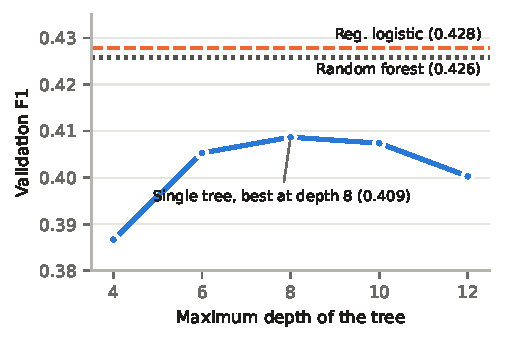
\includegraphics[width=0.8\linewidth]{tree_depth}
  \caption{Validation F1 of a single decision tree versus its maximum
  depth.}
  \label{fig:tree}
  \end{minipage}
\end{table*}

\textbf{Preprocessing.} Table~\ref{tab:ablation} shows that cleaning the
answer codes gives the largest gain (+0.013 F1): treating ``refused'' (9)
as a large number misleads a linear model. One-hot encoding and the
interactions each add a small improvement, while missing-value indicators
add 94 columns without any gain, so they were not kept.

\textbf{Linear models.} Table~\ref{tab:models} shows that the two logistic
models beat the four regression models: the squared loss also penalizes
confident correct predictions, unlike the logistic loss. Regularization barely
matters: with $N \gg D$ the model does not overfit, and $\lambda \geq
10^{-2}$ only lowers the F1. However, $X^\top X$ is singular (smallest
eigenvalue $\approx 0$) because several computed BRFSS variables are linear
combinations of others, so plain least squares produces very large weights
and ridge regression is the numerically stable choice. SGD needs a tiny
step because rare one-hot categories become very large after
standardization.

\textbf{Non-linear models.} A single tree is clearly worse than the linear
models (Fig.~\ref{fig:tree}): shallow trees underfit and deeper trees
overfit. Averaging 50 trees in a random forest almost closes the gap, and
averaging the forest with the logistic regression gives a small gain
(0.431). Boosting the logistic regression is the best model (0.436), confirmed by
5-fold CV ($0.4314 \pm 0.0040$ vs.\ $0.4268 \pm 0.0035$ for the logistic
regression): our hand-made products miss some interactions. The neural
network did not beat the linear models (0.417).

\textbf{Final model.} We submitted the regularized logistic regression
($\lambda = 10^{-4}$), retrained on all the training data with the
threshold chosen on the validation split ($t = 0.206$). Its 5-fold CV F1 is
$0.4268 \pm 0.0035$ (accuracy $0.871 \pm 0.007$, precision $0.35$, recall
$0.54$), and it obtained F1 $= 0.441$ and accuracy $= 0.878$ on AIcrowd,
our best leaderboard score. It finds about half of the sick persons, with roughly two
false alarms per true detection.

\section{Discussion}

We kept the model with our best leaderboard score. Boosting is the
most promising direction (+0.005 in CV). All
reasonable methods reach an F1 between 0.42 and 0.44, so the information in
the survey seems to be the main limit. The label is a past diagnosis, so
the model detects the disease rather than predicting it; strong predictors
such as difficulty walking may even be consequences of it.

\bibliographystyle{IEEEtran}
\begin{thebibliography}{1}
\bibitem{brfss}
Centers for Disease Control and Prevention, ``Behavioral Risk Factor
Surveillance System, 2015 survey data,''
\url{https://www.cdc.gov/brfss/annual_data/annual_2015.html}.
\bibitem{xgboost}
T.~Chen and C.~Guestrin, ``XGBoost: A scalable tree boosting system,'' in
\emph{Proc.\ KDD}, 2016, pp.~785--794.
\bibitem{adam}
D.~P.~Kingma and J.~Ba, ``Adam: A method for stochastic optimization,'' in
\emph{Proc.\ ICLR}, 2015.
\end{thebibliography}

\end{document}
